\paragraph{Evolutionary Origins of Morality}

Evolutionary biologists have proposed various mechanisms to explain how altruistic traits might evolve. Theories of kin selection~\citep{hamilton1964genetical} and reciprocal altruism~\citep{trivers1971evolution} show how limited forms of cooperation could evolve among relatives and repeated interaction partners. Recently, cultural group selection theories~\citep{boyd2011cultural, henrich2015secret} explain how groups with stronger moral norms outcompeted others, leading to the genetic evolution of psychological predispositions supporting moral behavior.
Evolutionary game theory provided mathematical frameworks demonstrating how cooperation can evolve under some strategies similar like previously mentioned mechanisms by showing strategies can yield higher payoffs than pure selfishness under specific conditions. \citet{nowak2006five}'s ``five rules for the evolution of cooperation'' identifies key mechanisms: kin selection, direct reciprocity, indirect reciprocity, network reciprocity, and group selection. 

Though these works provide great insights and a mathematical foundation for cooperation and moral evolution, they highly abstract away the rich complexity of human cognition and cooperation using mathematical models, blocking a full view of moral evolution dynamics.

\paragraph{Moral Frameworks}

% Our agent design draws upon descriptive moral frameworks that characterize the psychological and behavioral essence of morality. 
Moral Foundations Theory identifies five moral dimensions: care/harm, loyalty/betrayal, authority/subversion, and sanctity/degradation~\citep{Haidt2007MFT}. The Theory of Dyadic Morality~\citep{Gray2012TDM} emphasizes harm as the root of morality, while Morality-as-Cooperation theory~\citep{Curry2019MAC} identifies seven cooperative behaviors as essential: helping kin, helping group members, reciprocating, being brave, deferring to superiors, dividing resources fairly, and respecting others' property. Other theories ground morality in distinctions between rules and conventions~\citep{Turiel1983MDT}, social-relational models~\citep{Fiske1992RMT, Rai2011RRT}, specific moral emotions~\citep{Rozin1999CAD}, or an ethic of care~\citep{Gilligan1982EOC}.


While existing theories offer rich descriptions of morality's central traits, our initial investigation desires a framework that organizes these traits into scalable ``levels'' for a more systematic analysis. The Expanding Circle Theory~\citep{singer1981expanding} provides an ideal structure for this purpose. Its concept of a ``circle of concern'' that expands from the self, to kin, and finally to society offers a clear, tiered structure for defining an agent's moral level. Furthermore, this progression provides a natural way to integrate key concepts of other theories: care and loyalty are paramount within the kin circle, while fairness and reciprocity are essential for the stability of the broader group circle. This concentric model has cross-cultural relevance due to its deep resonance with philosophical traditions like Confucianism~\citep{fei1992from}, which also defines morality through the proper ordering of relational duties. Given its implementable structure and integrative power, we adopt the Expanding Circle as the primary theoretical foundation for our simulation.

\paragraph{LLM-Based Agent Simulation}

Recent advances in LLMs provide the methodological foundation for our approach to studying morality's evolution. LLM-based agent simulations can model entities with sophisticated cognitive architectures—including values, memory, perception, reasoning, and social dynamics—that generate emergent, complex behaviors~\citep{park2023generative, horton2023large}.
LLM agents allow for controlled experimentation with variables that would be impossible to manipulate in real-world settings; they provide transparent access to agents' decision-making processes; and they can simulate long timescales of social development~\citep{piao2025agentsociety}.

Prior work has demonstrated the versatility of this approach. \citet{park2023generative} created an interactive simulated small town where generative agents exhibited complex social behaviors, including relationship formation and collective problem-solving. \citet{horton2023large} applied LLM agents to economic simulations, finding that agents replicate known economic phenomena while providing unprecedented access to reasoning processes. \citet{aher2023using} validated that LLM agent simulations can reproduce results from human behavioral experiments, showing its potential as a complementary methodology in social science research.
However, existing environments lack the complete settings of agent morality, cooperative and competitive interactions, and evolution features, as demonstrated in Table~\ref{tab:comparison}.
One relevant recent work is ``Artificial Leviathan'', which explores social order in LLM agent societies, while they assume all agents are inherently selfish and focus on how social order emerges from this assumption~\citep{dai2024artificial}.

Therefore, by explicitly modeling agents with varying moral dispositions to better reflect the diversity of human moral psychology, our work represents the first systematic application of LLM-based simulations to investigate the evolution of morality in prehistoric human societies, where moral systems likely first emerged.

\begin{figure*}[t!]
    \centering
    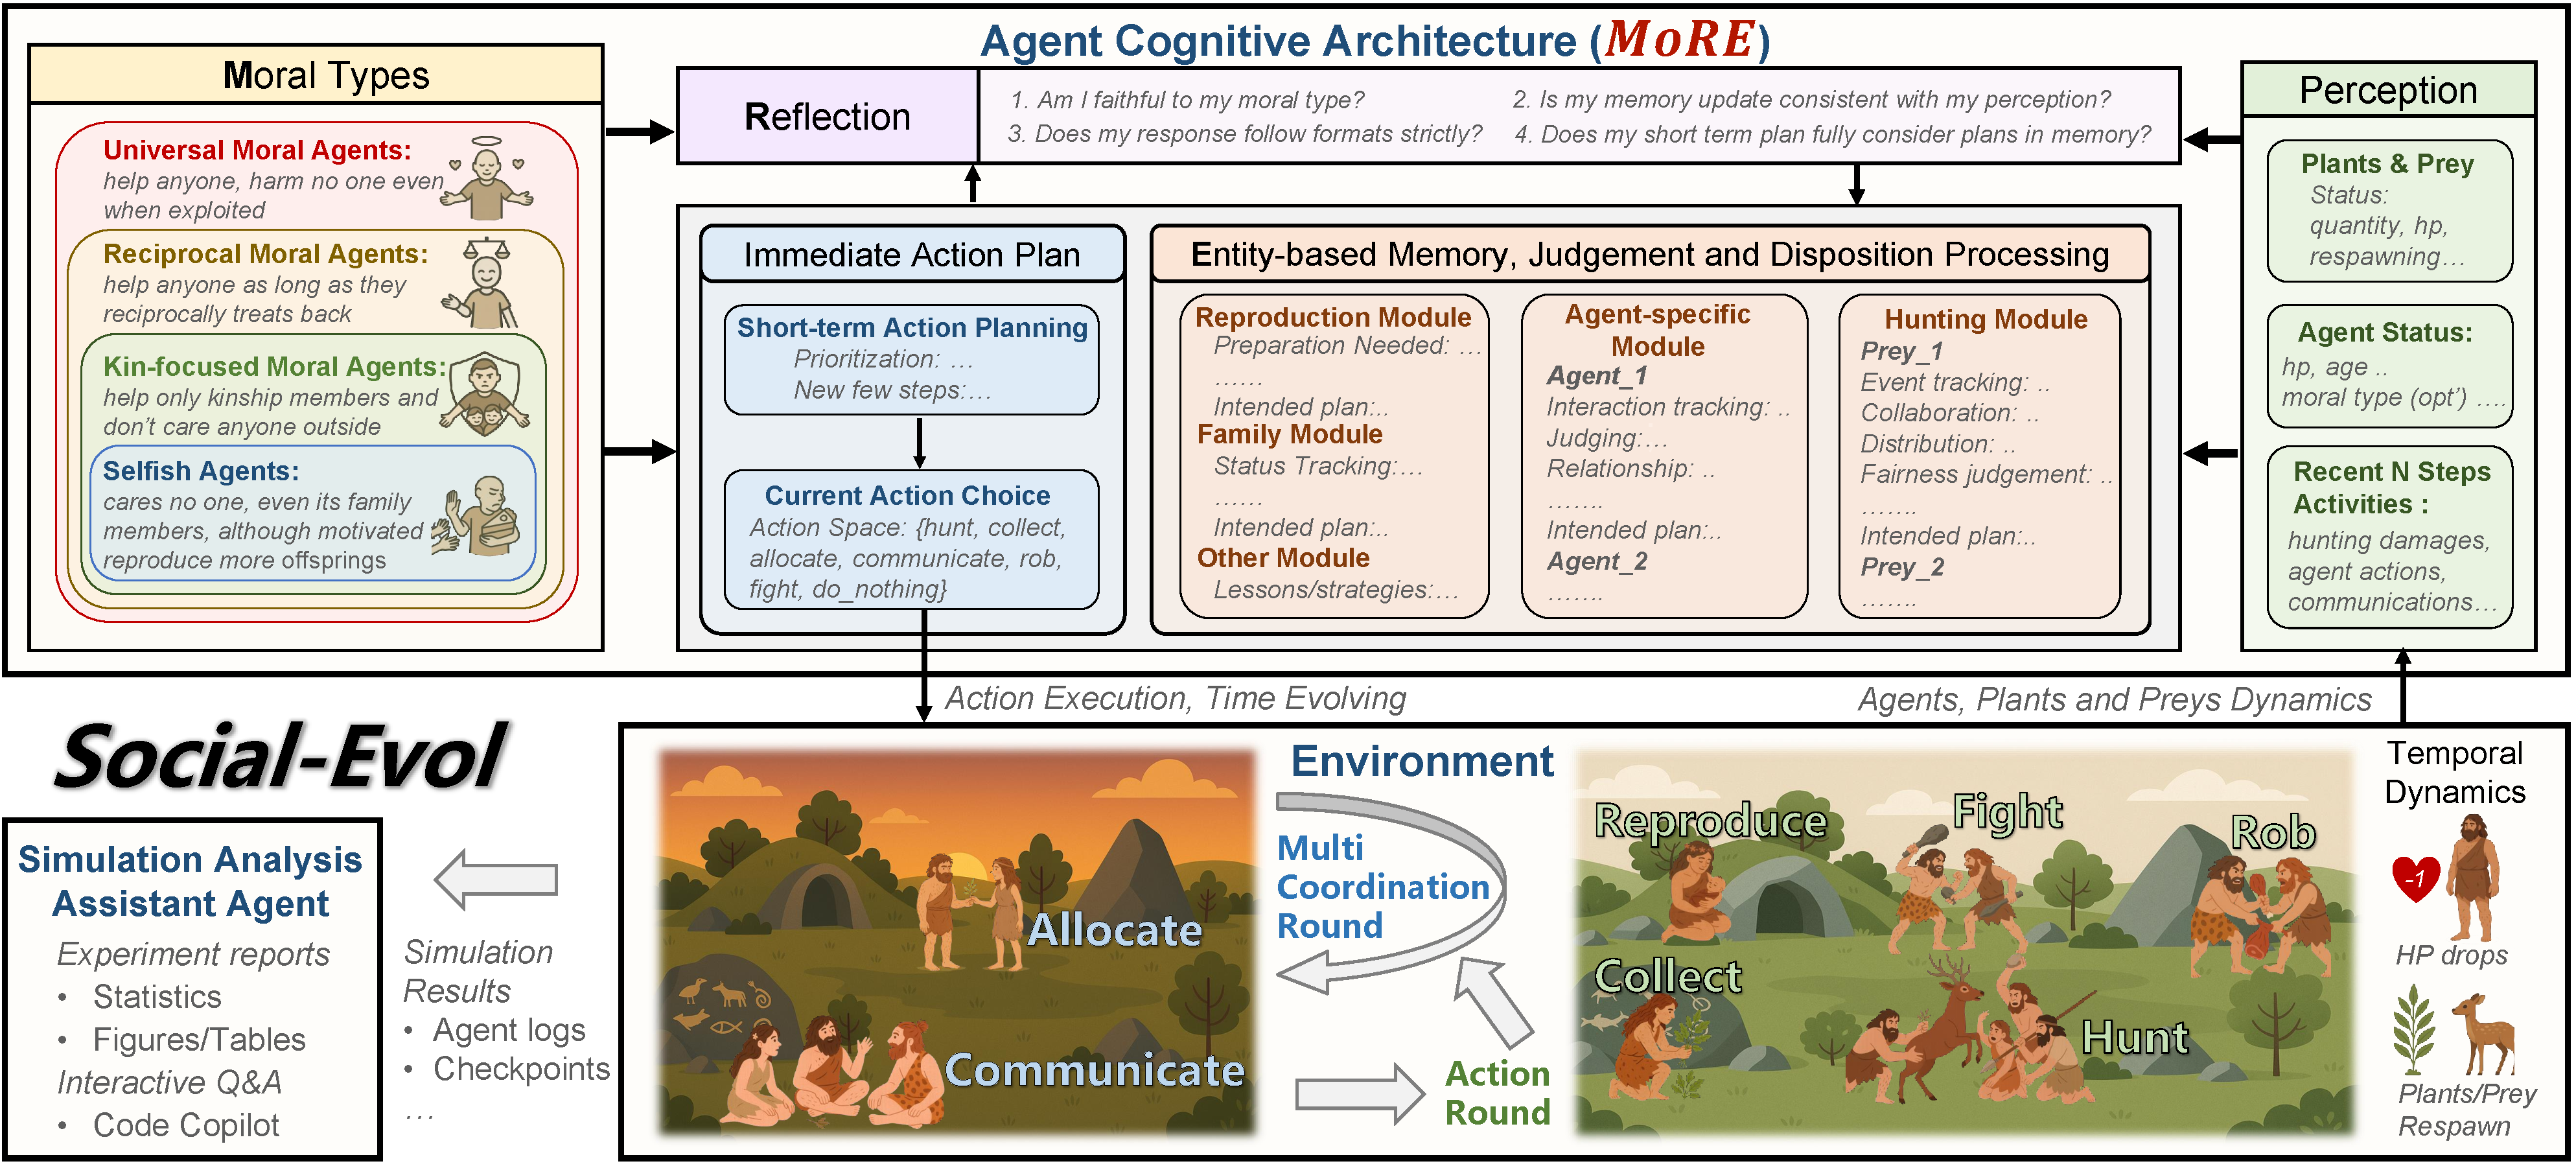
\includegraphics[width=0.95\textwidth]{figures/framework.pdf}
    \caption{Overview of our simulation framework. The \textit{Environment} follows defined temporal dynamics and iterates between (multi-)coordination rounds and action rounds to interact with agents. The \textit{Agent Cognitive Architecture} includes a moral value module prescribing moral types based on expanding circles of concern, a perception module processing environmental information, and cognitive modules that update memory, form judgments, and generate action plans consistent with the agent's moral type. Before execution, agents perform self-reflection to verify consistency with observed facts and moral dispositions. The \textit{Simulation Analysis Assistant Agent} is a developed tool to automatically analyze simulation results.}
    \label{fig:method}
\end{figure*}